\section{Background}
\label{chap:background}

3D Semantic Segmentation assigns semantic class labels to each element of a 3D data stream. All algorithms considered in this paper use Point Clouds as their data format, so our goal is to assign a label to each point in the cloud. It is not straightforward to apply 2D Semantic Segmentation algorithms to the 3D case for a number of reasons. One issue is that 3D data is sparse: while every pixel in an image has useful information, there are large sections of space in which even voxelized point clouds are completely empty. Another issue is the exponential growth of memory requirements and processing time required by adding another dimension. Finally, while cameras are ubiquitous and relatively easy to label, training 3D data has additional barriers to entry like sensor cost and the difficulty of training.

As in the 2D case it has become common practice to spur research into 3D Semantic Segmentation algorithms by publicly releasing labeled datasets, thus allowing research labs to try out their algorithms without needing to perform costly data collection and annotation. While this has certainly increased innovation, the complexities of 3D Semantic Segmentation make apples-to-apples comparison between segmenters a difficult task.

\subsection{Datasets}
\label{chap:datasets}

Datasets are collections of raw point cloud data along with per-point hand-labeled "ground truth" datum. No dataset is perfectly representative of the world, so it's important to test algorithms against as diverse a set as possible. Unfortunately, most segmentation algorithms only test their performance against one or two of the most popular publicly available datasets. Thus one goal of this projct is to see how state of the art algorithms perform against other, possibly more challenging, dataset.

We consider the datasets listed in Table \ref{tab:datasets}:
\begin{enumerate}
  \item SemanticKitti \cite{semantickitti1,semantickitti2}: One of the first publicly available datasets, SemanticKitti is the de facto data against which most algorithms test. This dataset features city driving in Germany with 28 semantic classes related salient to on-road autonomous driving.
  \item nuScenes \cite{nuscenes}: Released by Motional, this dataset is the second most popular available. It features complex city driving in Boston and Singapore, including driving in adverse weather conditions. nuScenes has 32 semantic classes salient to on-road autonomous driving.
  \item Rellis3D \cite{rellis3d}: A product of collaboration between the Army Research Lab and Texas A\&M University, this dataset considers the problem of offroad autonomy. 20 semantic classes are available which are useful in offroad driving.
\end{enumerate}

\begin{figure}[htp]
  \centering
  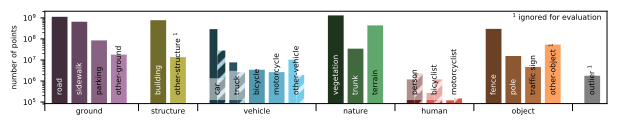
\includegraphics[width=0.7\textwidth]{images/semantic_kitti_label_distribution.png}
  \caption{SemanticKitti label distribution}
  \label{fig:semantickitti-label-distribution}
\end{figure}

\begin{figure}[htp]
  \centering
  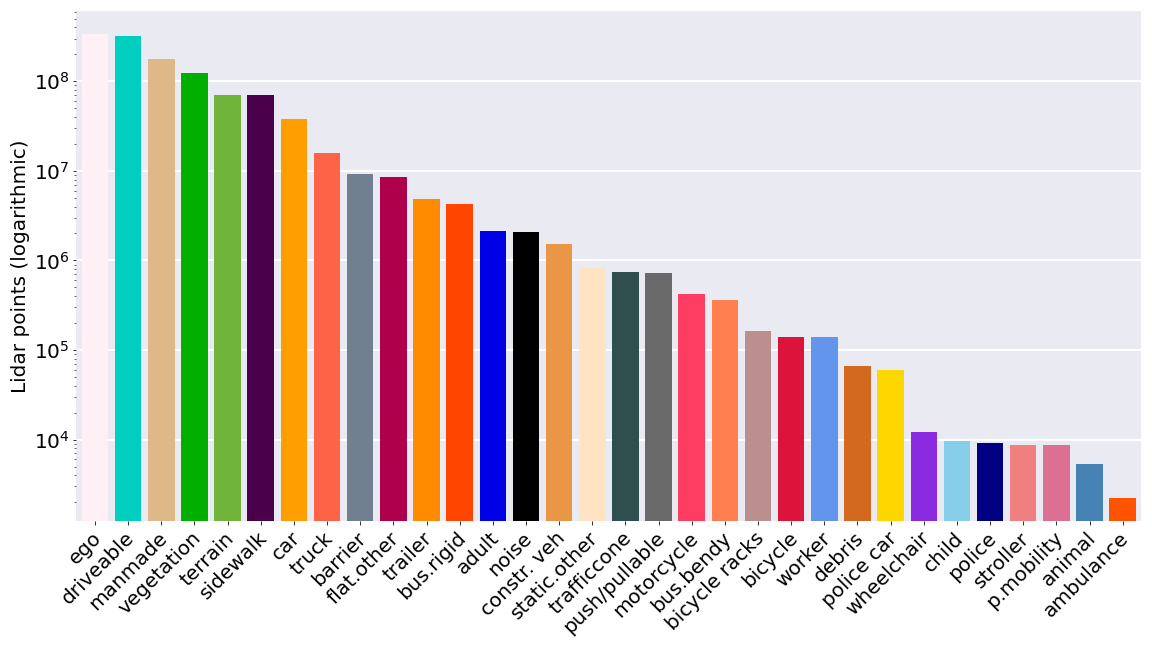
\includegraphics[width=0.7\textwidth]{images/nuscenes_label_set.png}
  \caption{nuScenes label distribution}
  \label{fig:nuscenes-label-set}
\end{figure}

\begin{figure}[htp]
  \centering
  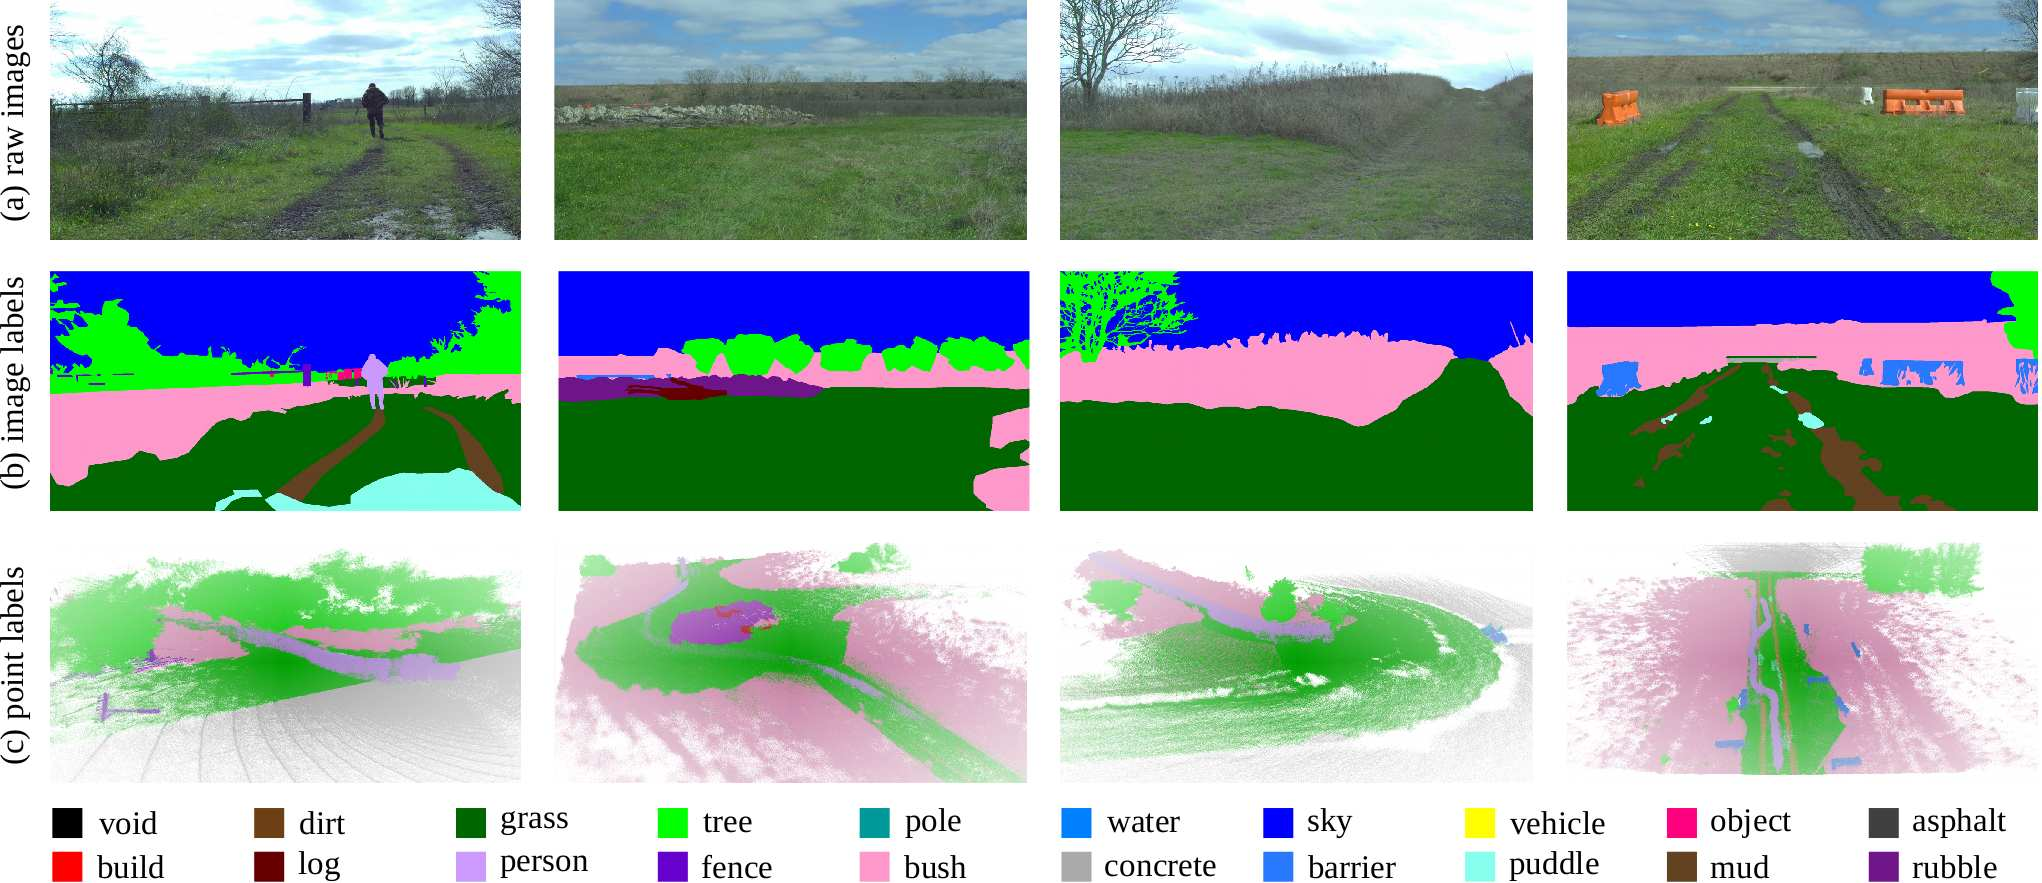
\includegraphics[width=0.7\textwidth]{images/rellis_label_suite.png}
  \caption{Rellis3D label distribution}
  \label{fig:rellis-labe-suite}
\end{figure}

\subsection{Segmenters}
\label{chap:segmenters}

There are many different approaches to the problem of 3D Semantic Segmentation \cite{deeplearningpcsurvey}. Some aim to get the best possible score for a given challenge using pure 3D data; others use multimodal fusion. Some are less focused on overall performance and instead attempt to make do with less data or less labeled data \cite{2dpass}. Some tackle the problem of sparsity with sparse convolution \cite{sparseconv}; others reject a voxelized representation in favor of pure point-based representations \cite{pointnet}. The sheer scale of this problem makes it impossible to choose a "best" algorithm. Although many of the algorithms considered in this project were chosen because they topped the ranking of a challenge, others were chosen as representative or interesting on the merit of their approach.

\begin{enumerate}
  \item SalsaNext \cite{salsanext}: A range-image based approach which was released in 2020 and benchmarked against SemanticKitti.
  \item Cylinder3D \cite{cylinder3d}: A cylindrical voxelization scheme is used in conjunction with sparse convolution in this 2020 paper which topped the leaderboards for both nuScenes and SemanticKitti.
  \item 2DPASS \cite{2dpass}: A multimodal approach which augments the 3D information with imagery. Released in 2022, this approach tops the SemanticKitti challenge as of this writing.
  \item COARSE3D \cite{coarse3d}: An approach to training which tackles the problem of limited annotations - this method trains against a limited subset of ground truth annotations via pixel anchors.
\end{enumerate}


\begin{figure}[htp]
  \centering
  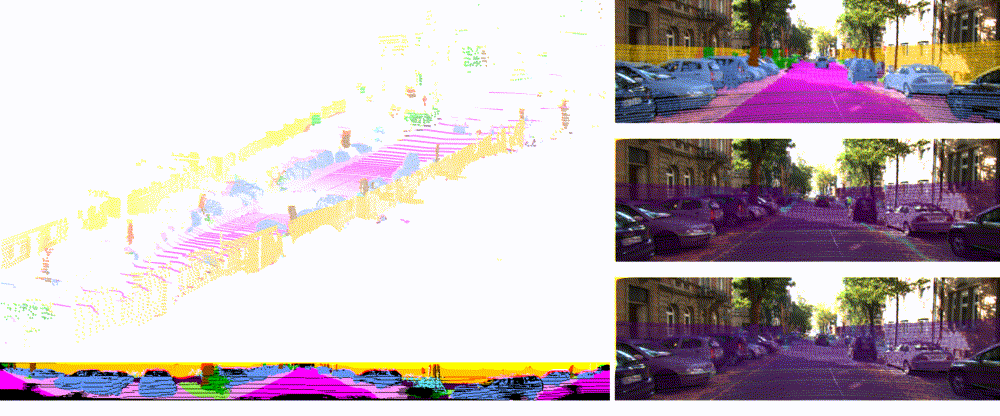
\includegraphics[width=0.7\textwidth]{images/salsanext_overview.png}
  \caption{SalsaNext overview}
  \label{fig:salsanext-overview}
\end{figure}

\begin{figure}[htp]
  \centering
  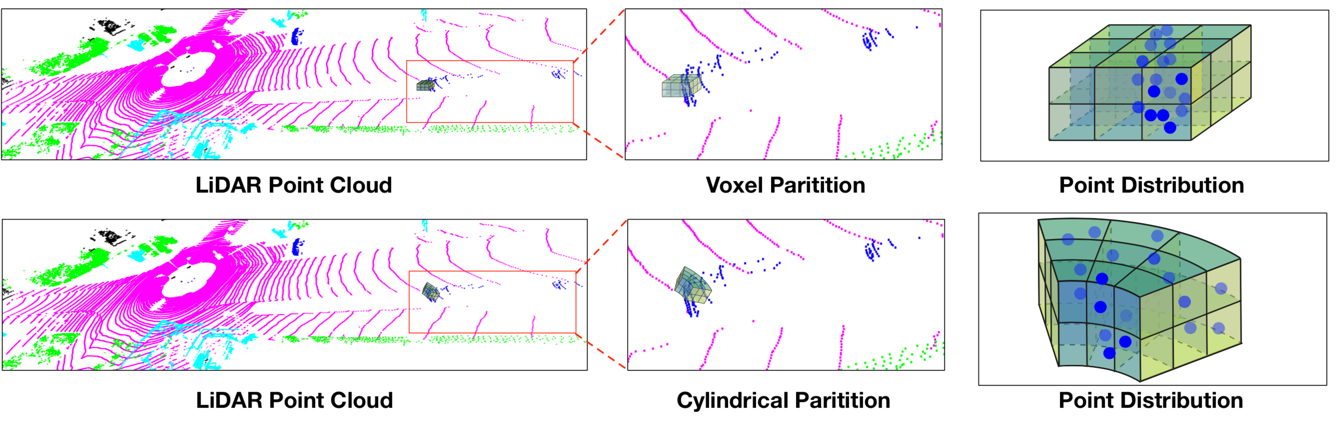
\includegraphics[width=0.7\textwidth]{images/cylinder3d_overview.png}
  \caption{Cylinder3D overview}
  \label{fig:cylinder3d-overview}
\end{figure}

\begin{figure}[htp]
  \centering
  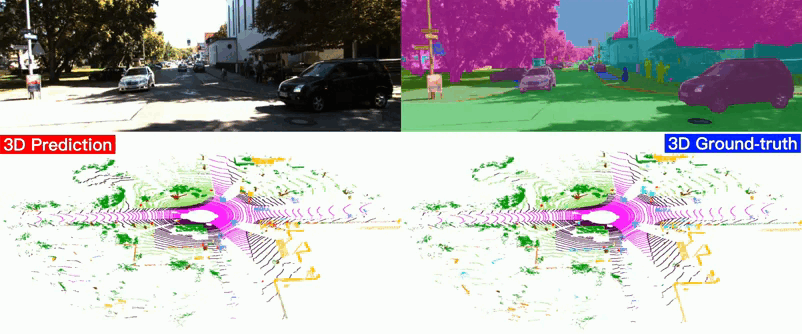
\includegraphics[width=0.7\textwidth]{images/2DPASS_overview.png}
  \caption{2DPASS overview}
  \label{fig:2dpass-overview}
\end{figure}

\begin{figure}[htp]
  \centering
  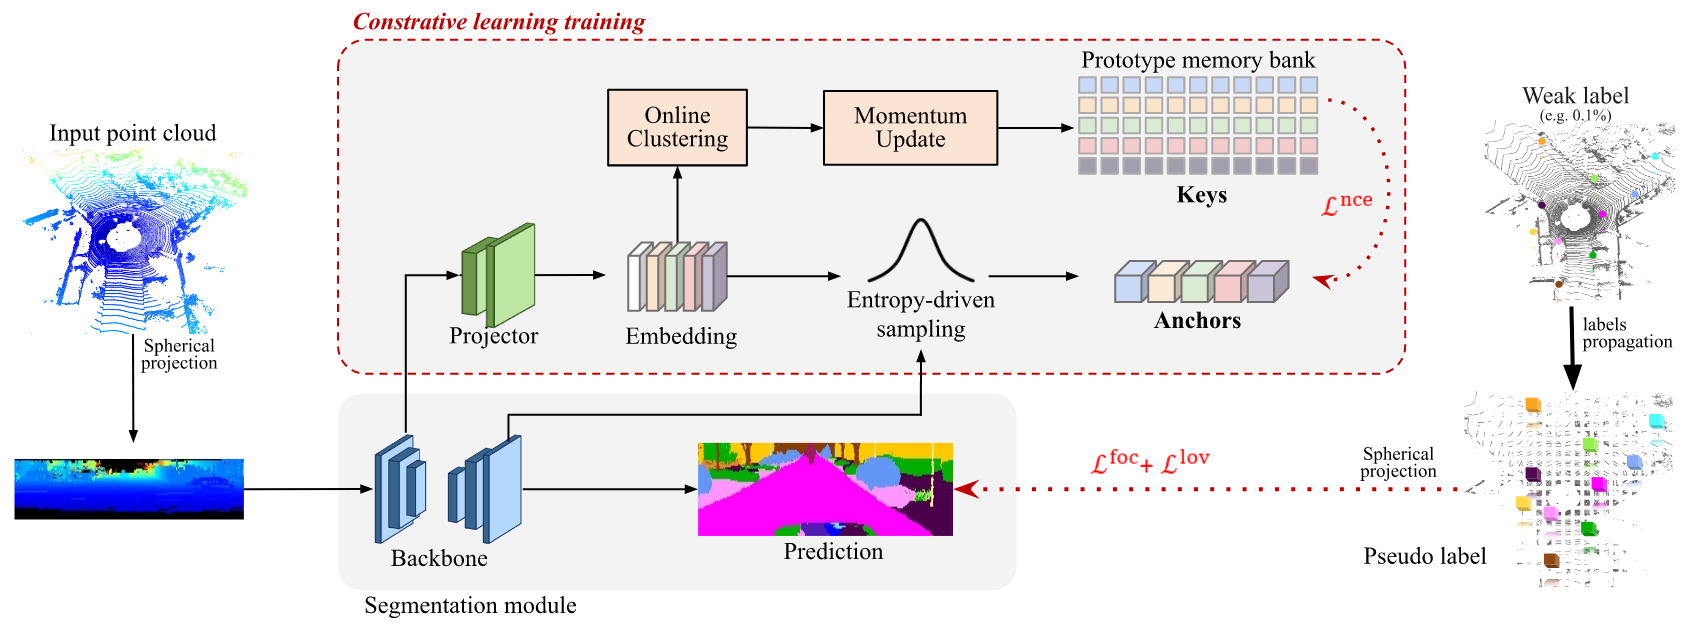
\includegraphics[width=0.7\textwidth]{images/coarse3d_overview.png}
  \caption{COARSE3D overview}
  \label{fig:coarse3d-overview}
\end{figure}

